\documentclass{article}
\usepackage{graphicx}
\usepackage{float}
\begin{document}

\title{GC Content in Yeast}
\date{2019\\November}
\author{Bo\v{z}ena Nevinskien\.{e}}
\maketitle

\section{First Section}
According to the literature, GC content of \emph{Saccharomyces cerevisiae} is 38.3\%. 
The goal of this study is to check if it is true. 
Also to determine if all yeast genes have the same GC content, and if not, why? 
For this study we randomly selected 3 strains or yeast and found their possible open reading frames:
\begin{enumerate}
	\item EC9-8: found 8622 possible open reading frames.
	\item VL3: found 9859 possible open reading frames.
	\item YS9: found 8341 possible open reading frames.
\end{enumerate}

In this study, we did not search for reverse complement open reading frames on the antisense DNA chain.                    
Also, not all reading frames may be accurate. The only criteria, that we followed is that the open reading frame must be
at least 50 codons in length between start codon (ATG) and stop codons (TAA, TAG and TGA).
After finding these ORFS, we calculated GC ratio in each of the ORFS and analysed frequency of GC ratios.


\subsection{EC9-8}

EC9-8 is a haploid cadmium-resistant derivative of a yeast isolated from the valley bottom of Evolution Canyon 
at Lower Nahal Oren, Israel.
The average of G and C nucleotides in EC9-8 yeast strain's possible ORFS was approximately 39.94\%.

\begin{figure}[H]
\vspace{30pt}%
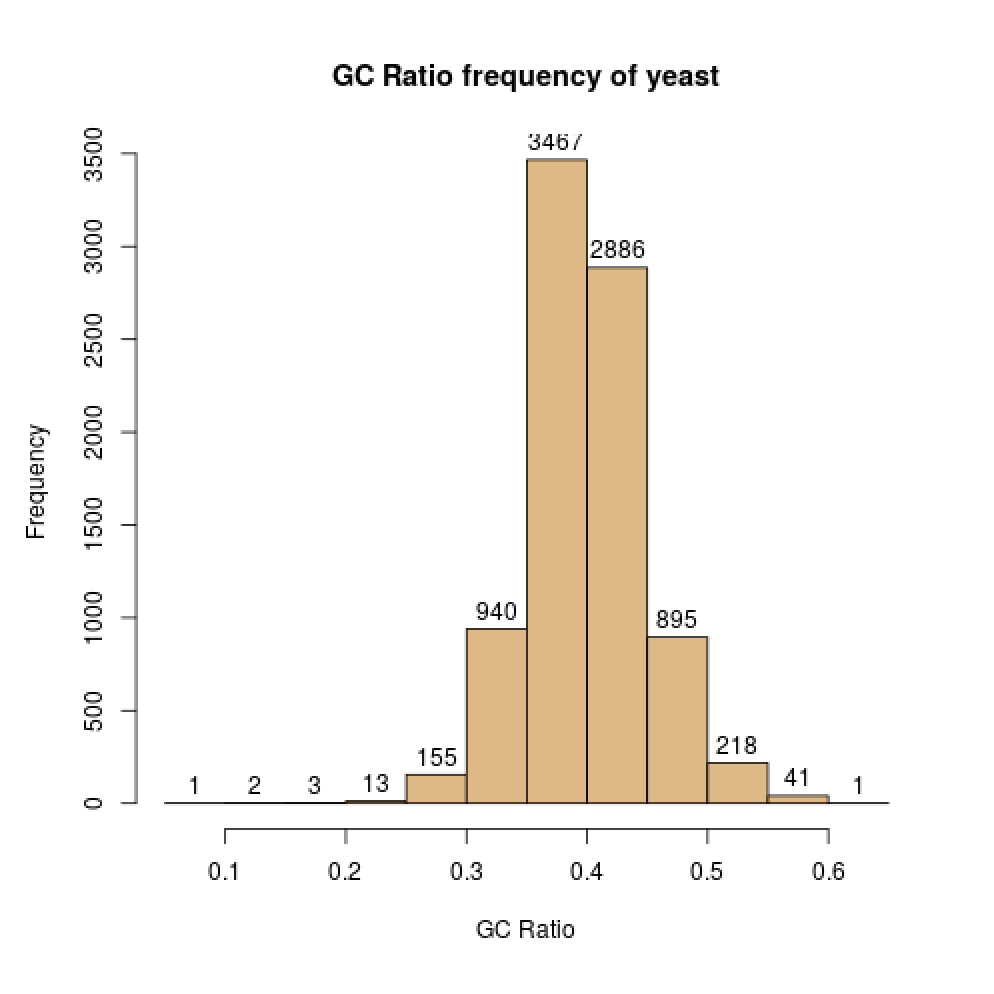
\includegraphics[width=50mm,scale=0.3]{images/EC9-8_ASinica_2011_AGSJ01000000.eps}
\caption{GC ratio in EC9-8 strain}
\label{fig:method}
\end{figure}

\subsection{VL3}

VL3 was isolated in Bordeaux, France, and is most suited to the production of premium aromatic 
white wines with high thiol content (citrus and tropical fruit characters). 
VL3 has a whole-chromosome amplification of chromosome VIII, as well as 54 ORFs that are missing in other strains.
The average of G and C nucleotides in EC9-8 yeast strain's possible ORFS was approximately 39.67\%. 

\begin{figure}[H]
\vspace{30pt}%
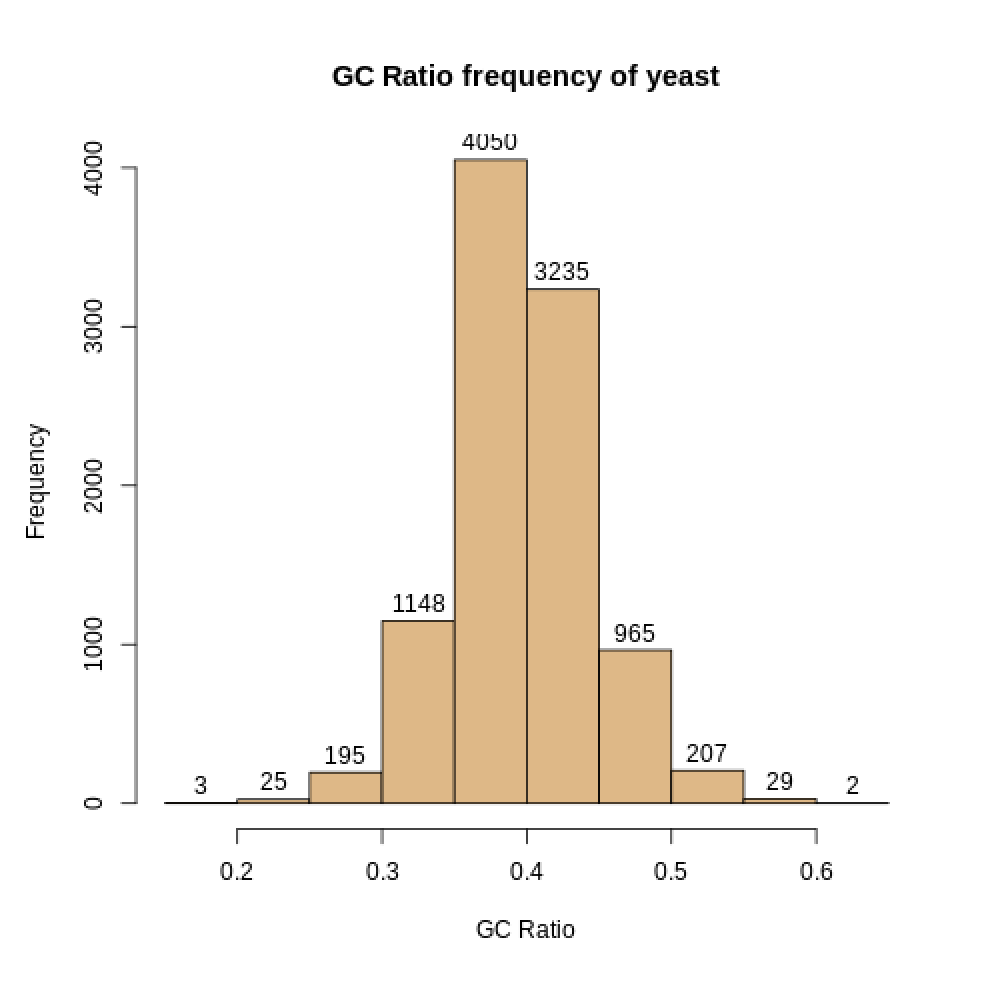
\includegraphics[width=50mm,scale=0.3]{images/VL3_AWRI_2011_AEJS01000000.eps}
\caption{GC ratio in VL3 strain}
\label{fig:method}
\end{figure}

\subsection{YS9}

YS9 is one of the Singapore's baking strains.
The average of G and C nucleotides in EC9-8 yeast strain's possible ORFS was approximately 39.97\%.

\begin{figure}[H]
\vspace{30pt}%
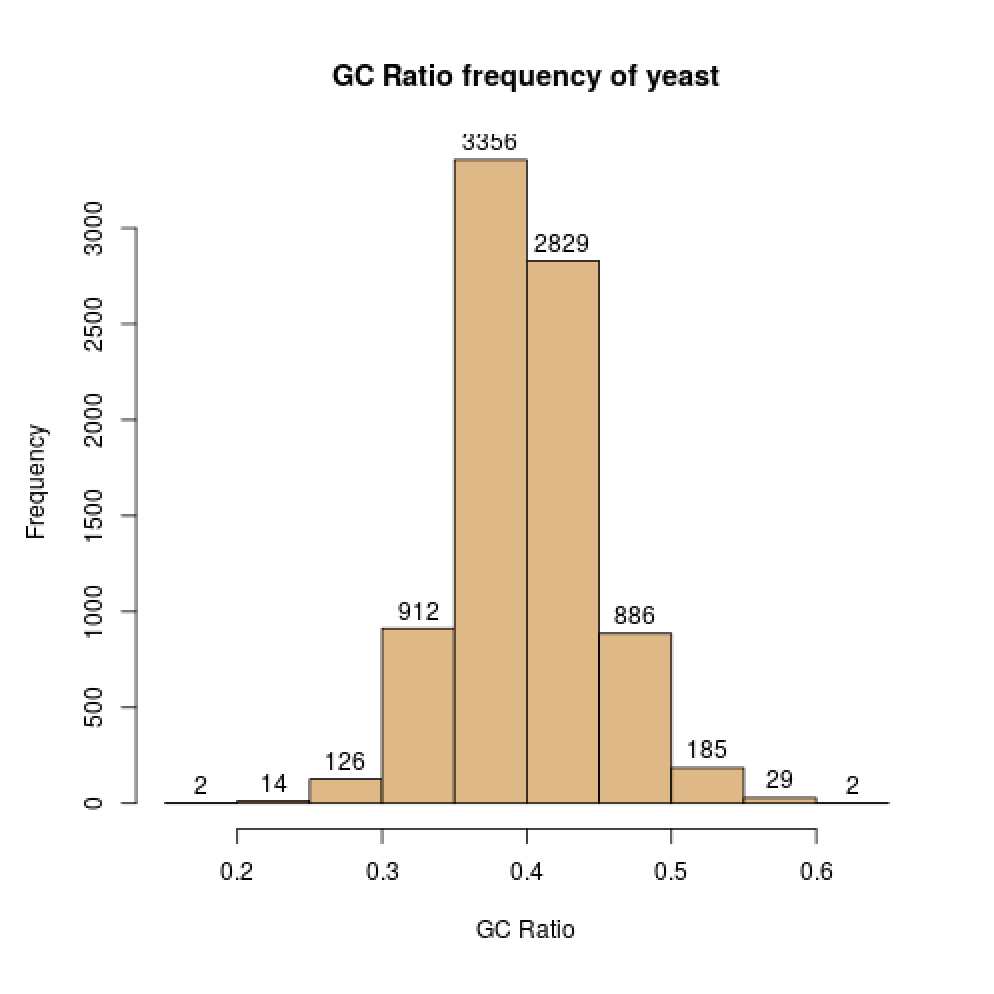
\includegraphics[width=50mm,scale=0.3]{images/YS9_Stanford_2014_JRIB00000000.eps}
\caption{GC ratio in YS9 strain}
\label{fig:method}
\end{figure}

Overall in all 3 strains the mean of G and C nucleotides was about 39.86\% of all nucleotides.
\begin{figure}[H]
\vspace{20pt}%
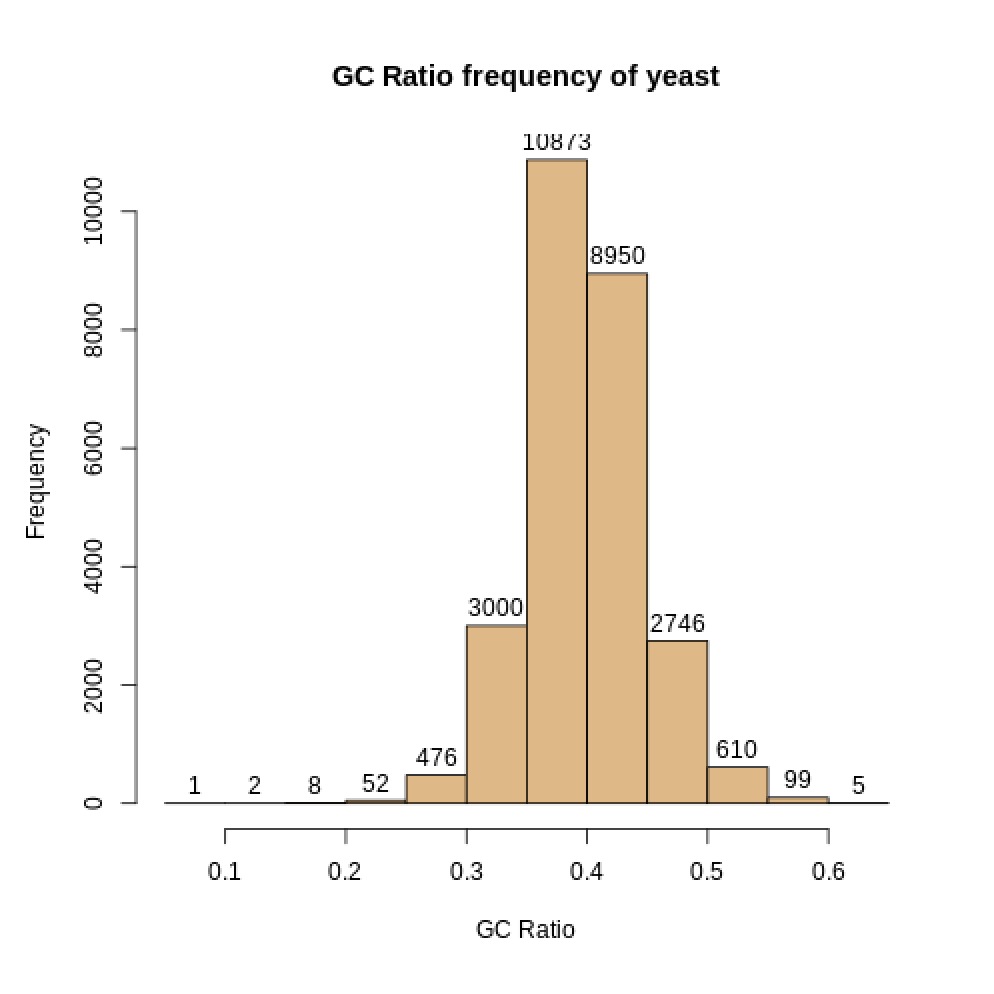
\includegraphics[width=50mm,scale=0.35]{images/AllGenomes.eps}
\caption{GC ratio in YS9 strain}
\label{fig:method}
\end{figure}
This work ...articles~\emph{some journal in italic} \cite{}.

\bibliographystyle{plain}
\bibliography{Citations.bib}

\end{document}
